\section{tasks::create\-Master\-Sky\-Flat Class Reference}
\label{classtasks_1_1createMasterSkyFlat}\index{tasks::createMasterSkyFlat@{tasks::createMasterSkyFlat}}
Inheritance diagram for tasks::create\-Master\-Sky\-Flat::\begin{figure}[H]
\begin{center}
\leavevmode
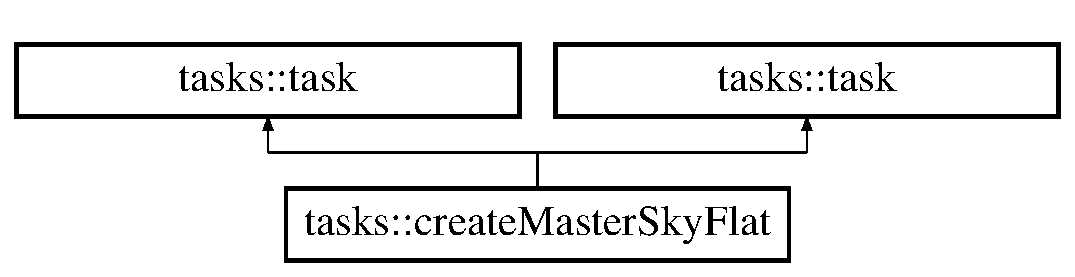
\includegraphics[height=2cm]{classtasks_1_1createMasterSkyFlat}
\end{center}
\end{figure}
\subsection*{Public Member Functions}
\begin{CompactItemize}
\item 
def \textbf{run}\label{classtasks_1_1createMasterSkyFlat_de8c1be37632c1836eaa04b9023e8051}

\item 
def \textbf{run}\label{classtasks_1_1createMasterSkyFlat_de8c1be37632c1836eaa04b9023e8051}

\end{CompactItemize}
\subsection*{Static Public Attributes}
\begin{CompactItemize}
\item 
string \textbf{name} = '{\bfcreate\-Master\-Sky\-Flat}'\label{classtasks_1_1createMasterSkyFlat_bf573809d89f30bf8f6f6570b318a569}

\item 
string \textbf{button\-Text} = 'Create Master Sky FLAT'\label{classtasks_1_1createMasterSkyFlat_0d4e6d50999b2b2617f91b4fbae9b4d6}

\item 
int \textbf{MIN\_\-NUMB\_\-FLATF} = 5\label{classtasks_1_1createMasterSkyFlat_584092cc9af81087d26b58d3a91efe0e}

\end{CompactItemize}


\subsection{Detailed Description}


\footnotesize\begin{verbatim}Create a master Sky FLAT from the Sky flatfield file list
\end{verbatim}
\normalsize
 



The documentation for this class was generated from the following files:\begin{CompactItemize}
\item 
old/PANICtool-1.0/tasks.py\item 
old/tasks.py\end{CompactItemize}
